\documentclass{article}% [Determines font size] { }Determines type of document (article/beamer/book/etc.)

\usepackage{graphicx}% Required package to compile figures.
\usepackage{blindtext}

\begin{document}% Required to produce a compiled LaTeX document. 

\blindtext

\begin{figure}[htbp]% h="here", t="top", b="bottom", p="page". 
        \caption{Complete figure format}% Creates a title for the figure, with an automatically generating ordered number placement of the figure. To place the title below the figure, then place the \caption command after \includegraphics.
        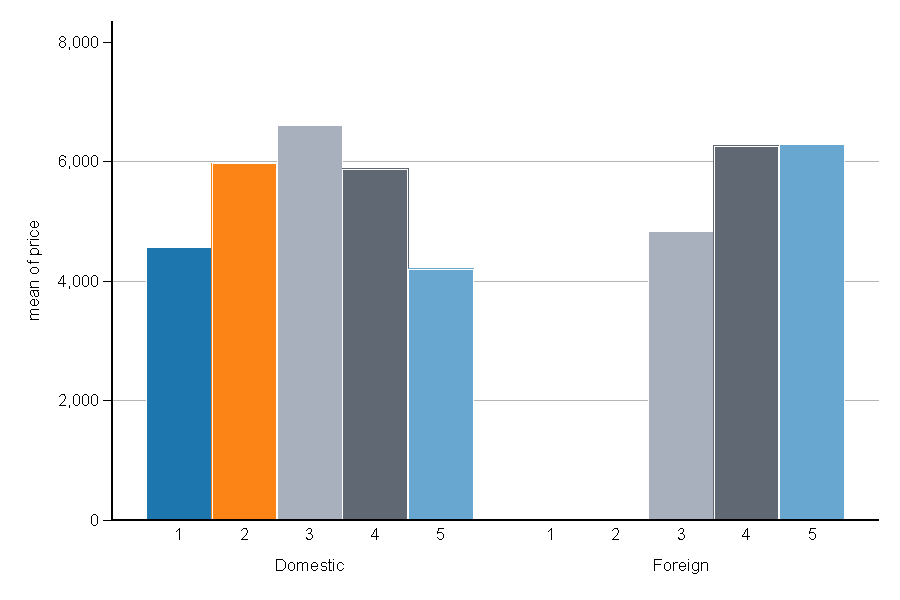
\includegraphics[width=1\textwidth]{figure1.pdf}% [ ] used to customize the size of the figure displayed in document. 
        \label{fig:placement_ht}%Use a ":" to create a category of labels on the left side, and the right side is the label of this specific figure.
\end{figure}

\begin{figure}[htbp]% Since this figure can't fit in the space below figure 1 on the same page (i.e. "h"), LaTeX then moves to the second option of "t" and places it at the top of next page and fills in the rest of the space in page 1 with the following text. 
        \caption{Complete figure format}% Creates a title for the figure, with an automatically generating ordered number placement of the figure. To place the title below the figure, then place the \caption command after \includegraphics.
        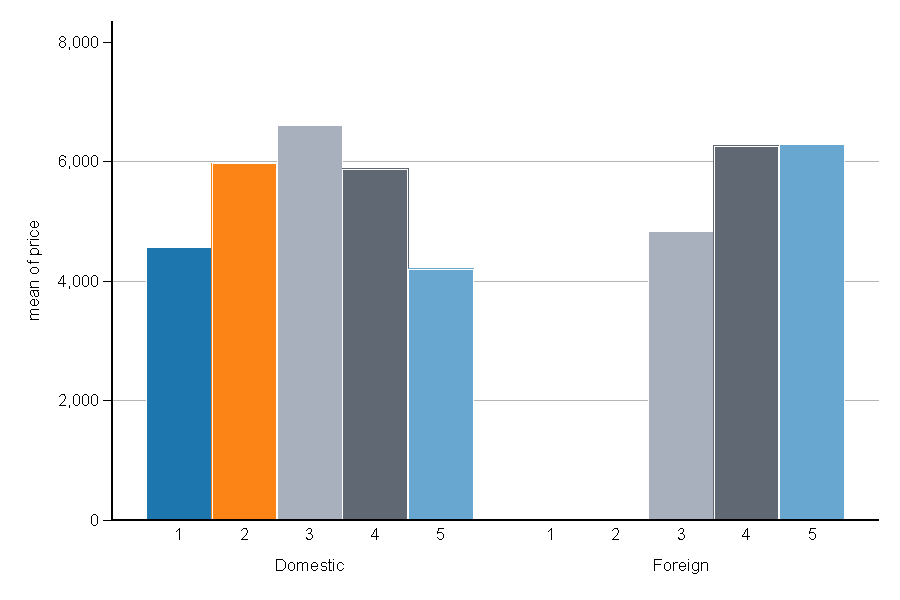
\includegraphics[width=1\textwidth]{figure1.pdf}% [ ] used to customize the size of the figure displayed in document. 
        \label{fig:placement_ht}%Use a ":" to create a category of labels on the left side, and the right side is the label of this specific figure.
\end{figure}

\blindtext[4]

\newpage

\end{document}